%versi 2 (8-10-2016) 
\chapter{Pendahuluan}
\label{chap:intro}
   
\section{Latar Belakang}
\label{sec:label}

Internet merupakan jaringan yang menghubungkan berbagai macam perangkat yang memungkinkan pertukaran informasi secara cepat. Pertukaran informasi di internet diatur oleh sebuah protokol. Protokol tersebut adalah TCP/IP(\textit{Transmission Control Protocol/Internet Protocol}). Informasi yang diberikan oleh penyedia informasi tentunya harus mudah dimengerti oleh orang yang mengakses informasi tersebut. Informasi yang mudah dimengerti tidak hanya dalam bentuk tulisan, namun bisa juga berupa gambar, video, atau suara. Kebutuhan inilah yang menyebabkan munculnya layanan \web yang berjalan di atas internet.

Layanan \web(\textit{World Wide Web}) memiliki protokol HTTP(\textit{HyperText Transfer Protocol}) sebagai aturan dalam pertukaran informasi yang dilakukan. Layanan \web ini dibangun dengan menggunakan berbagai teknologi yang ada, dalam perkembangannya banyak bermunculan pihak ketiga yang memberikan layanan berupa teknologi untuk membuat halaman web dari segi \textit{front end} maupun dari segi \textit{back end}, beberapa contoh dari teknologi tersebut adalah PHP, JavaScript, dan MySQL. Perkembangan teknologi ini kemudian dicatat oleh sebuah situs bernama \textit{HTTP Archive}.

Situs \web \textit{HTTP archive} ini mencatat perkembangan teknologi yang dipakai dalam membuat \web. Situs ini mencatat perkembangan penggunaan teknologi berdasarkan beberapa kriteria seperti pengalaman pengguna dalam menggunakan \web, kecepatan sebuah \web dalam memuat informasi, dan tingkat aksesibilitas sebuah \web. Dalam penelitian ini aspek yang akan diamati dari perkembangan teknologi pembuatan \web adalah CrUX(\textit{Chrome User Experience}). Aspek ini mengukur tingkat interaktif dan lamanya sebuah \web dalam memuat informasi berdasarkan pengalaman nyata pengguna Chrome dengan kondisi yang bervariasi.

Data yang telah didapatkan dari situs \web \textit{HTTP archive} ini disimpan ke dalam sebuah layanan penyimpanan data berbasis \textit{cloud} yang dikembangkan oleh Google yaitu \textit{Google Big Query}. Layanan ini memungkinkan penggunanya untuk memproses data dengan menggunakan \textit{query SQL}. SQL sendiri merupakan bahasa pemrograman untuk mengelola \textit{big data}. SQL juga memiliki fungsi untuk menyimpan, mengubah, menghapus, dan mengambil data dalam sistem manajemen basis data.

        \begin{figure}[]
        \centering
        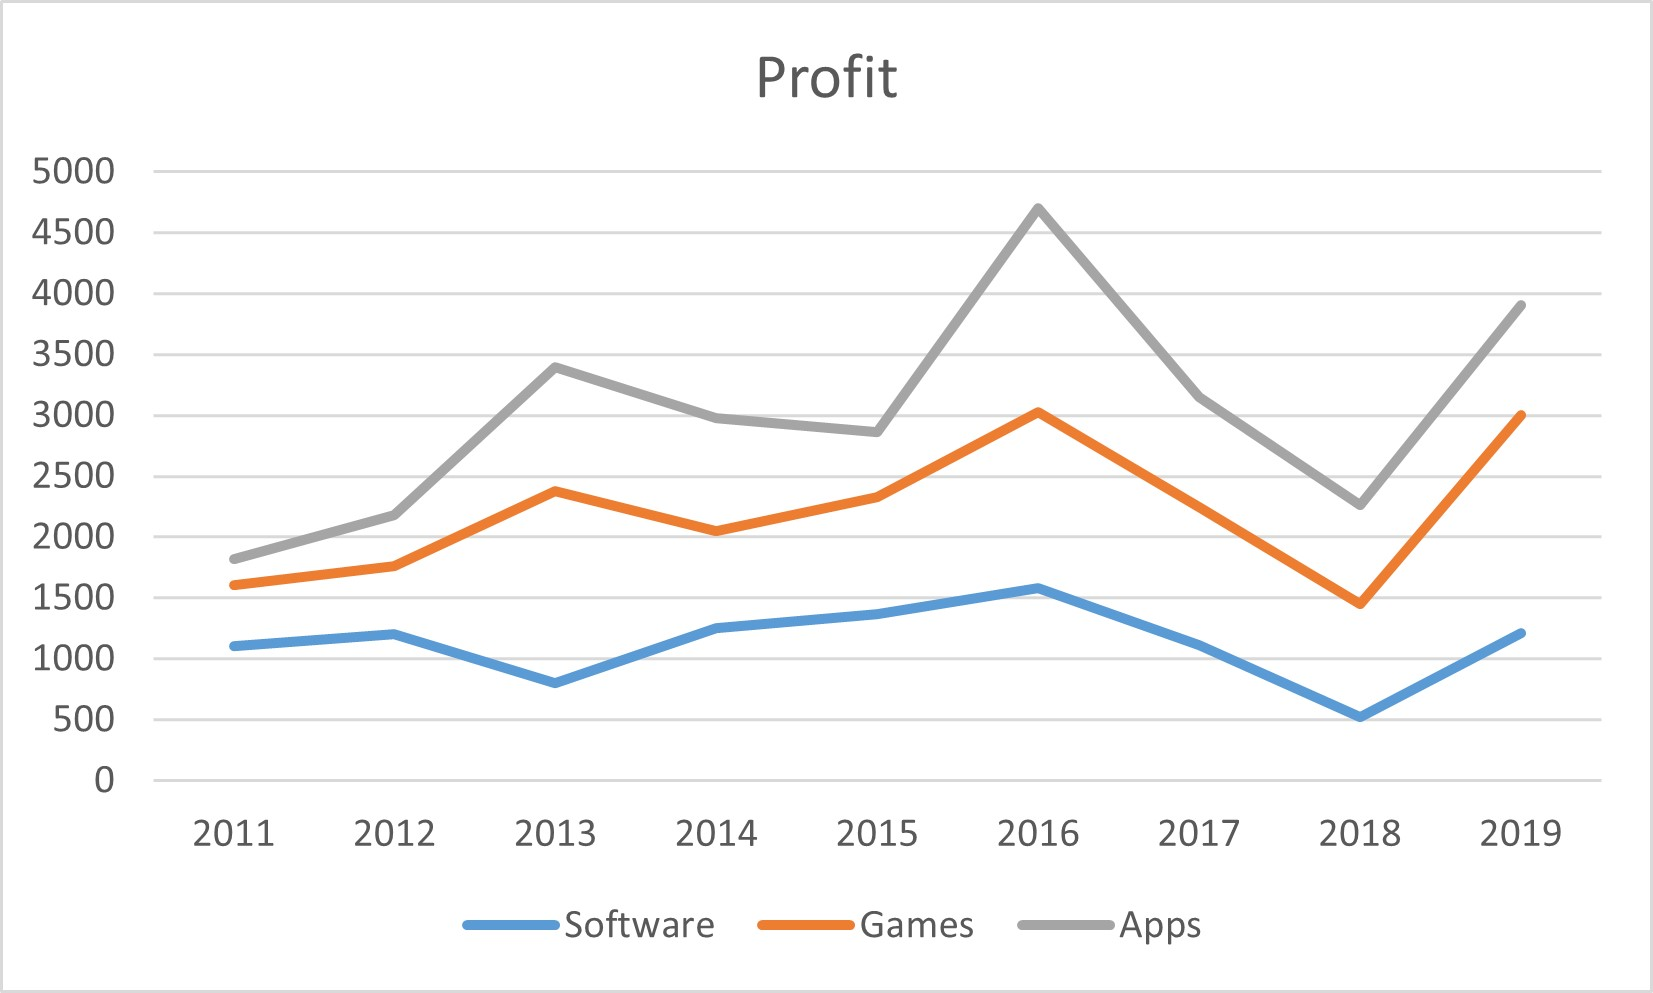
\includegraphics[width=0.5\linewidth]{Gambar/contoh linechart.jpg}
        \caption{Contoh \textit{line chart}}
        \label{fig:contohlinechart}
    \end{figure}

    Data perkembangan ini kemudian disajikan dalam bentuk visualisasi agar lebih mudah dimengerti. Salah satu bentuk visualisasi yang dapat digunakan untuk menjelaskan perkembangan ini adalah \textit{line chart}. Contoh \textit{line chart} dapat dilihat pada gambar~\ref{fig:contohlinechart}\footnote{Gambar didapatkan dari \url{https://www.simonsezit.com/article/how-to-make-a-line-graph-in-excel/}}. Visualisasi ini dapat memperlihatkan perkembangan secara jelas dengan rentang waktu yang lebih lebar. Hal ini berguna karena data yang digunakan adalah data dari 60 bulan terakhir atau data dari bulan oktober 2018 hingga bulan desember 2024.
    
\section{Rumusan Masalah}
	Rumusan masalah yang akan diselesaikan dalam penelitian ini adalah:
    \begin{enumerate}
        \item Bagaimana perkembangan teknologi pembuatan \web selama 60 bulan terakhir?
        \item Bagaimana pekembangan teknologi pembuatan \web yang banyak digunakan oleh pembuat \web?
        \item Bagaimana cara menyajikan pekembangan teknologi pembuatan \web kepada pengguna?
    \end{enumerate}
	
\section{Tujuan}
	Tujuan yang akan dicapai dari penelitian ini adalah:
    \begin{enumerate}
        \item Mengetahui perkembangan teknologi pembuatan \web selama 60 bulan terakhir.
        \item Mengetahui perkembangan teknologi pembuatan \web yang banyak digunakan oleh pembuat \web.
        \item Membuat perangkat lunak untuk menyajikan perkembangan teknologi pembuatan \web.
    \end{enumerate}
\section{Batasan Masalah}
\label{sec:batasan}
Batasan masalah yang diterapkan pada penelitian ini adalah sebagai berikut:
\begin{enumerate}
    \item Data yang digunakan berasal dari rentang 60 bulan terkahir. Hal ini dimaksudkan untuk membatasi ukuran data agar tidak besar.
    \item Data yang akan dianalisis adalah data jumlah penggunaan dan persentase penggunaan. Hal ini dilakukan agar cakupan analisis tidak terlalu besar.
\end{enumerate}

\section{Metodologi}
\label{sec:metlit}
Metodologi yang digunakan dalam melakukan penelitian ini adalah sebagai berikut:
\begin{itemize}
    \item Mengumpulkan data penggunaan teknologi pembuatan \web selama 60 bulan terakhir.
    \item Membersihkan data dari kolom dan baris yang tidak digunakan.
    \item Melakukan analisis dengan menggunakan data dengan skala lebih kecil.
    \item Melakukan analisis dengan menggunakan data yang sebenarnya.
    \item Membuat GUI untuk menampilkan hasil analisis secara interaktif.
\end{itemize}

\section{Sistematika Pembahasan}
\label{sec:sispem}
Sistematika pembahasan tugas akhir ini adalah:
\begin{enumerate}
    \item Bab 1: Pendahuluan
   
    Membahas latar belakang, tujuan, rumusan masalah, batasan masalah, dan metodologi penelitian yang digunakan.
    
    \item Bab 2: Landasan Teori

    Membahas \web, \textit{HTTP Archive}, bahasa SQL, \textit{Google Big Query}, dan visualisasi data yang digunakan.

    \item Bab 3: Analisis Masalah

    Membahas tentang analisis masalah dan solusinya dan melakukan analisis dengan menggunakan data yang skalanya lebih kecil.

    \item Bab 4: Penambangan Data
    
    Membahas eksplorasi dan analisis data dengan menggunakan data \textit{real}.

    \item Bab 5: Pembuatan GUI dan Peluncuran Model

    Membahas tentang pembuatan GUI dan pengujian fungsional GUI untuk menampilkan hasil anlisis secara interaktif.

    \item Bab 6 : Kesimpulan dan Saran

    Membahas tentang kesimpulan dari hasil penelitian yang telah dilakukan dan saran agar peelitian ini lebih baik.
\end{enumerate}
